Hvis man, med utgangspunkt i eksponensiell forsterker, bytter plasseringen
til motstanden og dioden får man en logaritmisk forsterker.

\begin{figure}[H]
  \caption{Logaritmisk forsterker}
  \centering
  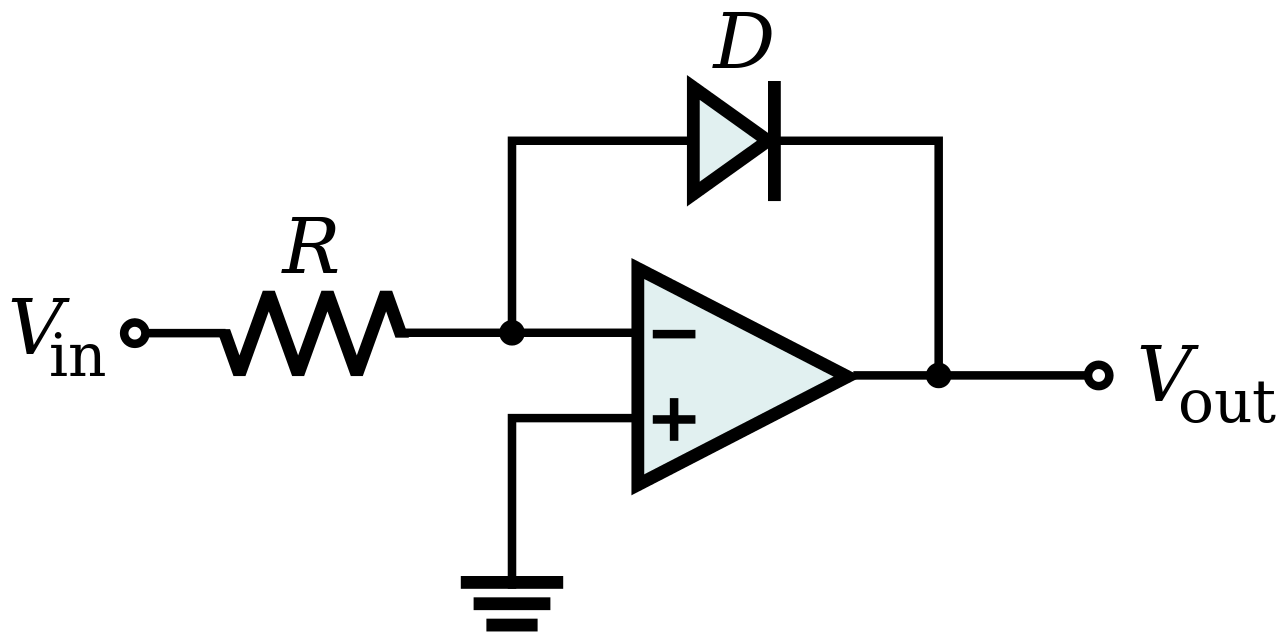
\includegraphics[width=0.5\textwidth]{./img/logamp}
\end{figure}

Spenningen ut er gitt ved
$$v_o = -V_T \cdot \ln{v_s}$$
